% auteur: Dorian VOLPE

\begin{frame}
	\frametitle{\textit{Hashed Timelock Contract} (HTLC)}
	\begin{itemize}
		\item Ne nécessite pas de tiers de confiance.
		\item Se base sur deux primitives.
		      \begin{itemize}
			      \item Un verrou temporel.
			      \item Un verrou de hachage.
		      \end{itemize}
		\item Utilisé pour des échanges sur la même blockchain puis rendu possible et maintenant largement utilisé pour des échanges \textit{cross-chain}.
	\end{itemize}
\end{frame}


\begin{frame}
	\frametitle{HTLC utilisation}

	\begin{figure}[h!]

		\stackunder{
			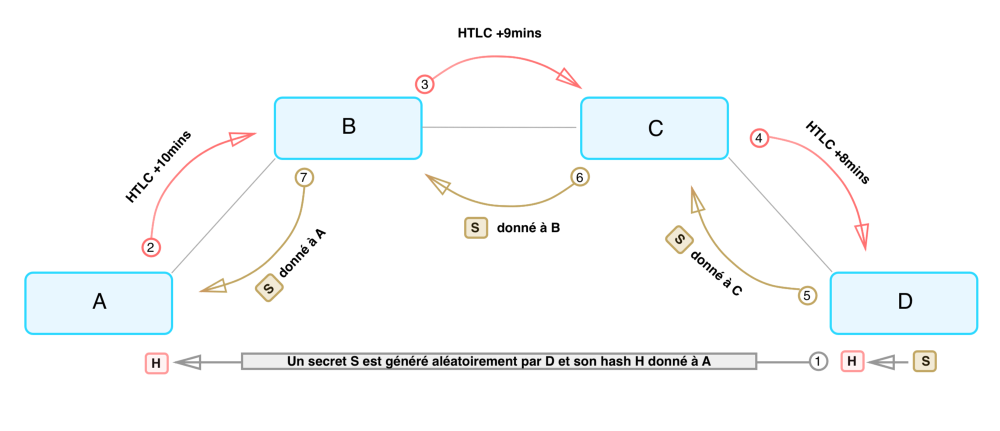
\includegraphics[scale=0.35]{decentralisation/Timed-HashLocks-Diagram-Image.png}}
		{\scriptsize
			Source: \url{https://www.coinhouse.com}}
	\end{figure}

\end{frame}

\begin{frame}
	\frametitle{Atomic Swaps}
	Un swap atomique permet un échange de cryptomonnaies de blockchains séparées
	\begin{itemize}
		\item Effectué entre deux entités sans l’intervention d’un tiers de confiance.
		\item L’idée est de supprimer les intermédiaires centralisés comme les échanges réglementés et de donner aux propriétaires de jetons un contrôle total.
		\item Utilise les HTLC. \newline
	\end{itemize}
	Deux propriétaires de cryptoactifs acceptent d’échanger leurs jetons pour une quantité donnée
	$\Rightarrow$ notion de connecteur publique.
\end{frame}

\begin{frame}
	\frametitle{Atomic Swaps - Exemple}
	\begin{figure}
		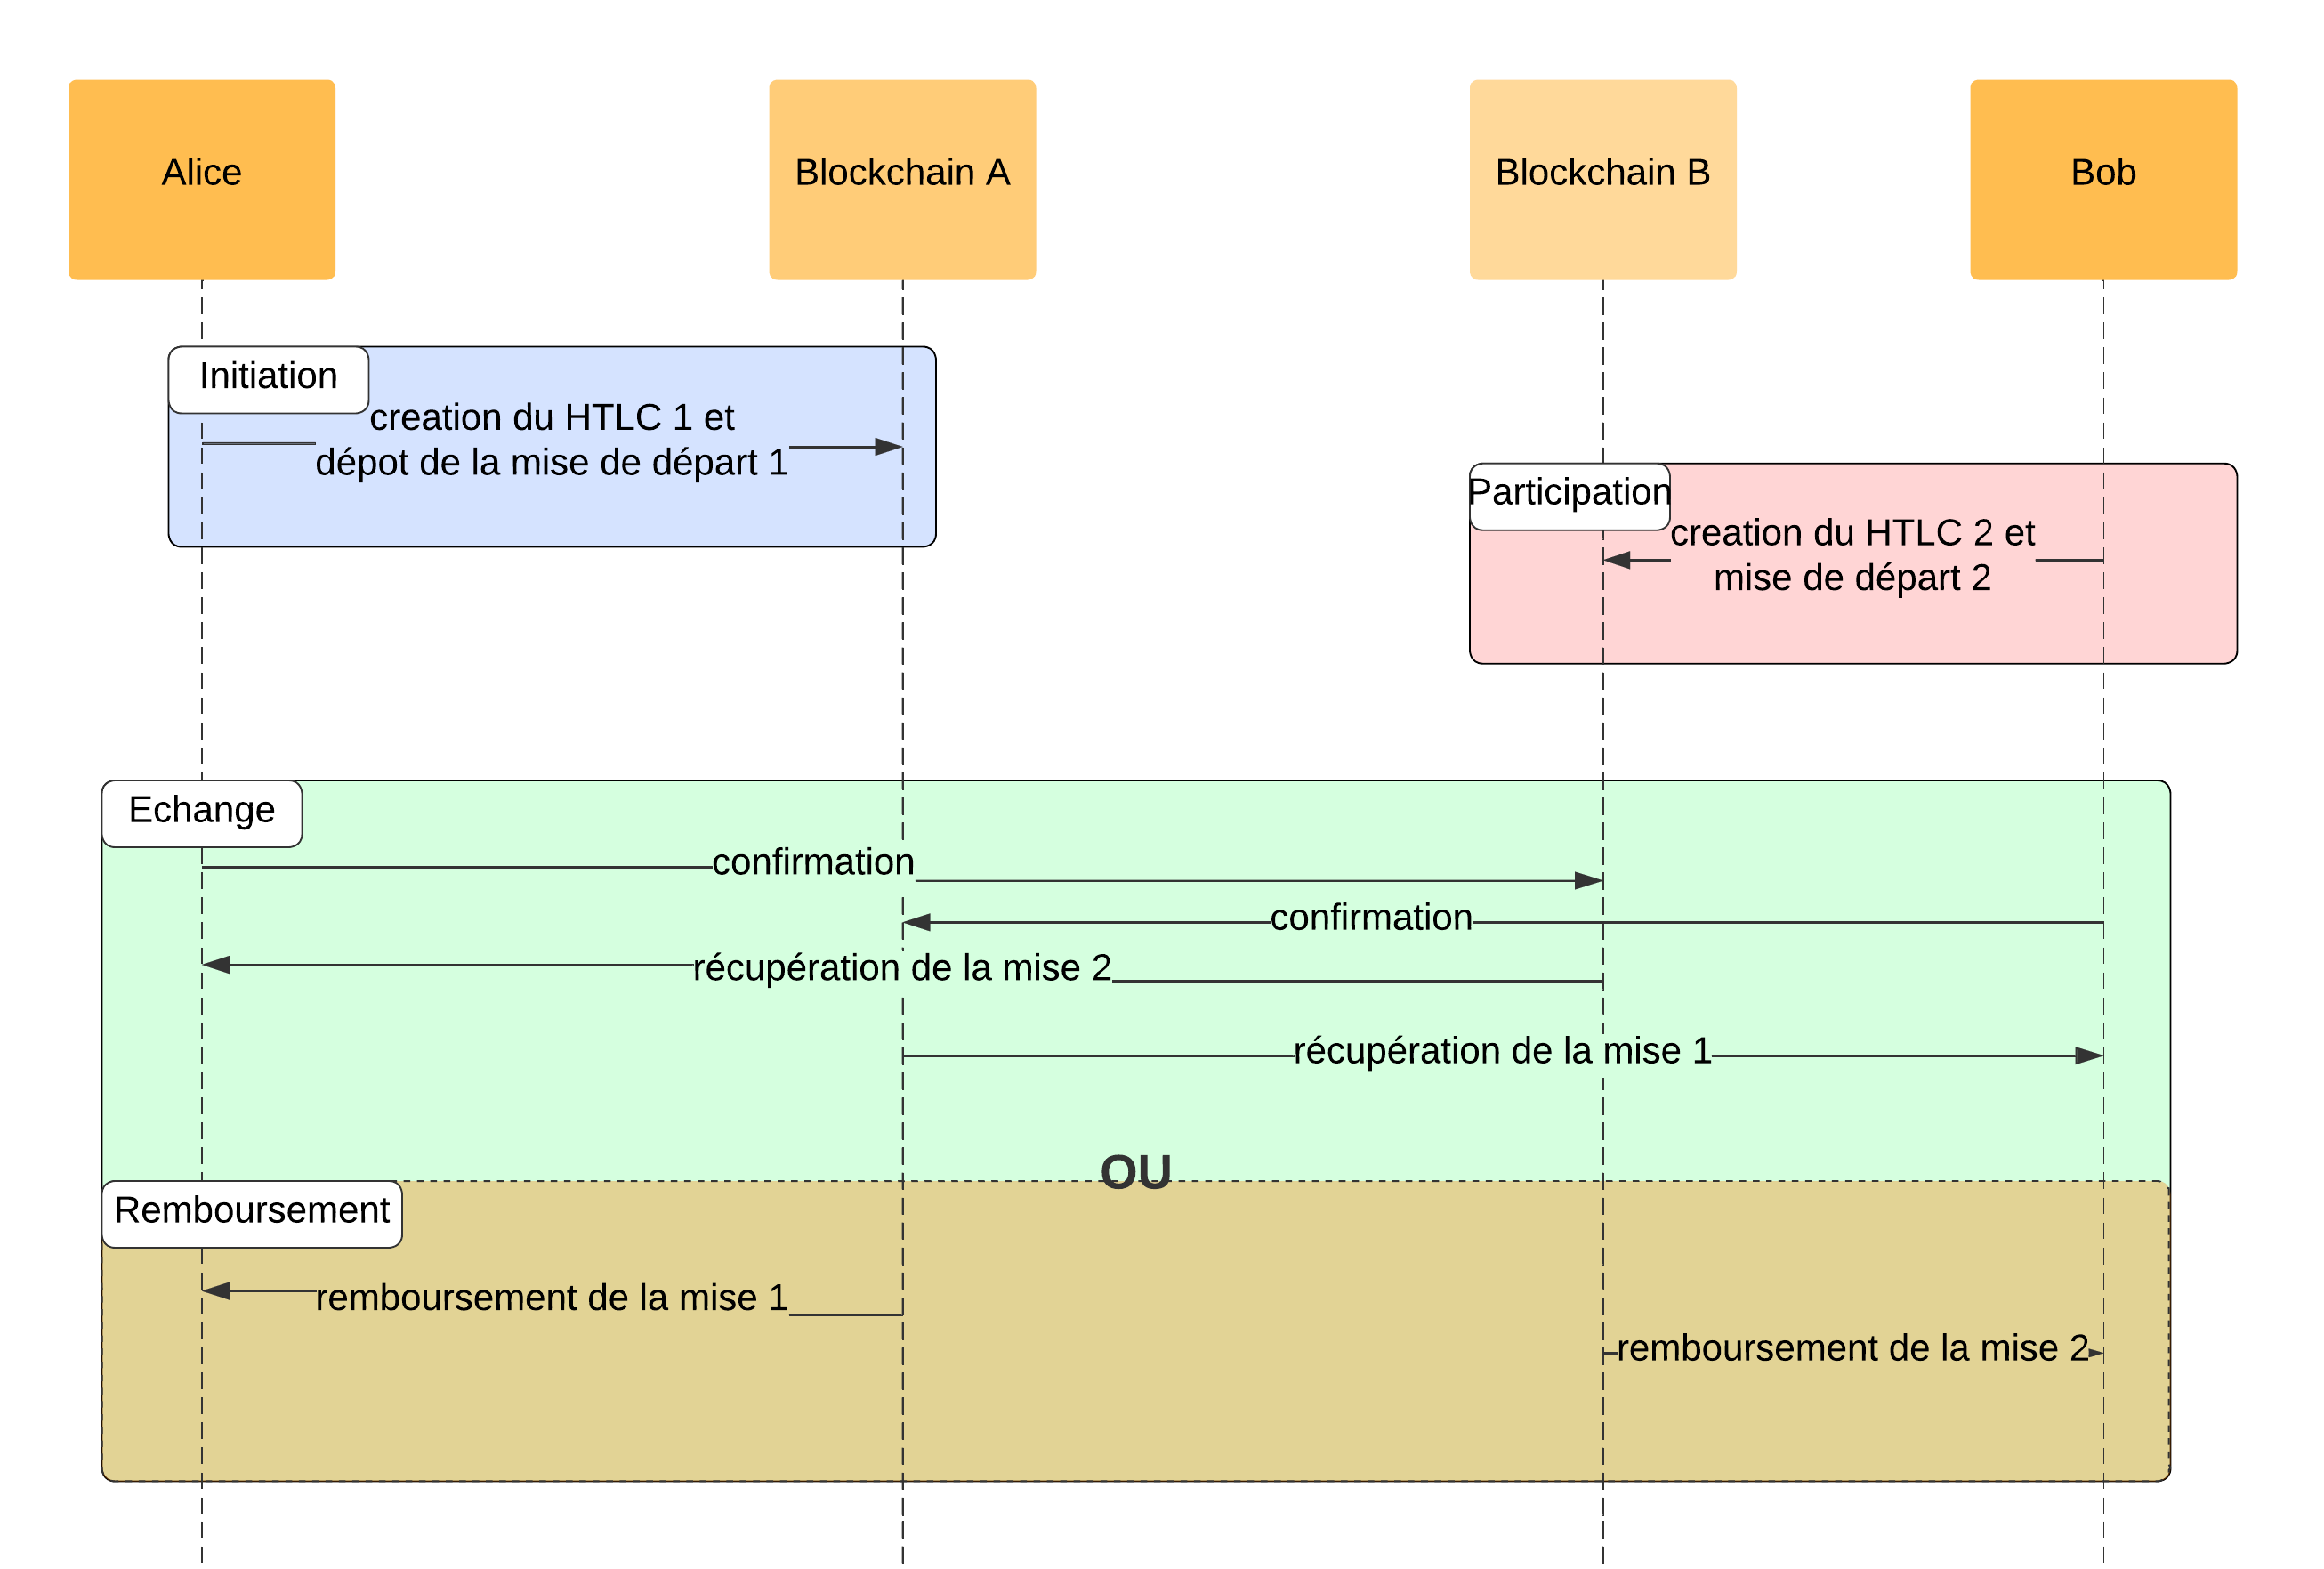
\includegraphics[scale = 0.10]{decentralisation/atomicSwap.png}
		\caption{Processus d'échange atomique avec HTLC}
	\end{figure}

\end{frame}

\begin{frame}
	\frametitle{Atomic Swaps - Avantages}
	\subtitle{Avantages}
	\begin{itemize}
		\item Réduction des coûts de transaction.
		\item Échange pair à pair sans tiers de confiance $\Rightarrow$ réellement décentralisé.
		\item Protection des échanges:
		      \begin{itemize}
			      \item Si un tiers suit le protocole il est assuré de ne pas perdre d'argent.
			      \item Si jamais il ne suit pas le protocole il perd sa mise.
		      \end{itemize}
	\end{itemize}
\end{frame}

